\section{Brugergrænsefladen} \label{brugergraenseflade}
Det er besluttet at systemet bliver implementeret som en hjemmeside.
I dette afsnit forklares de generelle designprincipper, som brugergrænsefladen er pålagt på vores hjemmeside.
Først beskrives en række forskellige guidelines, der ofte benyttes på hjemmesider, både til mobilt og desktop brugergrænseflader.
Derefter diskuteres de valg, der er taget ved nogle af vores hjemmesides elementer, samt hvordan det opfylder de nævnte guidelines.
Derefter fremvises det, hvordan den responsive brugergrænseflade er implementeret vha. Twitter Bootstrap, med kodeeksempler. 

\subsection{Teori}
Der findes forskellige teknikker at designe hjemmesider efter, og hermed også forskellige begreber, der benyttes i forbindelse med design af en brugergrænseflade.
Ifølge \citep{DIS2014} er de følgende tre elementer vigtige i denne forbindelse:
\begin{itemize}[nolistsep,noitemsep]
	\item \textbf{Learnability}
	\item \textbf{Effectiveness}
	\item \textbf{Ease of use}
\end{itemize}

Learnability kan opfyldes vha. \textbf{affordance} og \textbf{consistency}.
Affordance betyder her, at noget er designet, så det er tydeligt hvad det skal bruges til.
For eksempel at en knap er designet, så det ser ud som om, den kan trykkes på. 
På den måde giver affordance et intuitivt design, hvor brugeren kan regne ud, hvordan ting skal inteageres med.
Consistency betyder her, at hvis en opgave udføres på en måde et sted, bør den også udføres sådan et andet sted.
Der findes flere måder at opnå learnability på, men dette er to gode metoder, der mindsker mængden af viden, der kræves for at benytte hjemmesiden.

Effectiveness kan opfyldes vha. \textbf{recovery}, og/eller \textbf{constraints}.
Recovery betyder her, at hvis man laver en fejl, eller farer vild, skal det være nemt at komme tilbage, eller rette fejlen man lavede.
Constraints betyder her at forhindre brugeren, i at gøre noget de ikke burde, såsom at lave store fejl. 
Dette kan undgås ved at mindske mulighederne i forskellige skærmvinduer, eller f.eks. ved at spørge: ``Er du sikker på du vil slette dette?''.

Ease of use kan opfyldes vha. \textbf{navigation} og \textbf{feedback}.
Navigation betyder her at brugeren får assistance til at vide, hvor de befinder sig.
Dette kan f.eks. opnås med såkaldte breadcrumbs, der viser stien, som brugeren har bevæget sig ud af.
Feedback, betyder her at brugeren føler, at deres handlinger har gjort noget; derved er de ikke i tvivl om hvorvidt det f.eks. er nødvendigt at trykke på den samme knap en gang til.

Det er desuden relevant at gruppere felter på en brugergrænseflade, for at vise der et sammenhæng. 
Her kan benyttes en af Getalts love om perception, f.eks. proximity, eller continuity.\citep{DIS2014}

\textbf{WIMP}\hfill\\
En generel hjemmeside falder ind under begrebet WIMP, som er en type brugergrænseflade.
Det står for \textit{Windows}, \textit{Icons}, \textit{Menus} og \textit{Pointers}.
Vinduerne(\textit{Windows}) indkapsler forskellige data og aktioner, man kan interagere med på hjemmesiden, som f.eks. at tilgå opskrifter, eller en indkøbsliste.
Ikoner(\textit{Icons}) bruges til at illustrere mulige handlinger og emner.
Her kan benyttes forskellige designs til ikonerne, såsom direct-mapping, metaforer, eller convention.
Menuer(\textit{Menus}) bruges til at navigere på hjemmesider f.eks. imellem vinduerne, eller forskellige handlinger der skal udføres.
Pointeren(\textit{Pointers}) er et redskab, der bruges på hjemmesiden, og er på en almindelig pc ofte en markør, og på mobiltelefoner bruges touch-skærme, hvor ens fingre fungerer som pointere.


\textbf{Mobilt interface}\hfill\\
På en enhed med en mindre skærm, f.eks. en smartphone er der mindre plads til information, end på en f.eks. en computer. 
En række principper er defineret af Google\citep{Mobil}, og deres hovedpunkter er:
\begin{itemize}[nolistsep,noitemsep]
	\item Design hele hjemmesiden til at være mobilvenlig.
	\item Benyt et responsivt design så domænet forbliver det samme.
	\item Brugere på en mobilside vil have opnået deres mål hurtigt. Design derfor efter konteksten hvori mobilsiden bruges, og design efter dette, uden det går udover indholdet.
\end{itemize}

I næste sektion vil vi diskutere, hvordan disse elementer skal benyttes på hjemmesiden, for at udvikle en brugervenlig hjemmeside.

\subsection{Design}
For at kunne øge hjemmesidens ease of use, skal der bruges et redskab til at navigere rundt på hjemmesiden.
Dette kan f.eks. gøres vha. menuer med hierarkier, eller vha. en navigerings-bar i toppen.
Der vælges at bruge en navigerings-bar, af Bootstrap klassen navbar. 
På hjemmeside på mobilen kan det være uhensigtmessigt at bruge en menu hierarkier, derfor er en navbar med direkte links til komponenterne god at bruge. 
Den er vist overalt på hjemmesiden, og er derfor nem at navigere.
Ud for alle emner på navigerings-baren er der et ikon, så brugeren nemmere kan genkende funktionerne på menupunkterne.
Dette hjælper desuden også på sidens consistency, da denne altid er vist.

For at sikre sig learnability på siden, er det de samme klasser fra Bootstrap, der benyttes over alt på siden. 
Knapperne der har samme funktion, f.eks. som at tilføje noget til en indkøbsliste er ens over det hele. 
Det er et plus ikon, som ændrer sig til et flueben når der trykkes på den.
Denne feedback forsikrer brugeren om, at deres handlingen er udført.
Dette er konventionen, et plus lægger noget til, og et flueben viser at hændelsen er sket.
På samme måde angiver et kryds i en rød firkant, at man lukker noget ned, eller sletter noget.

Vælger brugeren at slette hele indkøbslisten eller en opskrift, bliver de præsenteret for en besked, der advarer dem om sletningen og den manglende mulighed for at gendanne.
Denne advarelse eksiterer dog ikke for at fjerne ting fra nævnte lister.
Der er desuden sat forskellige constraints for brugeren, således at en mængde ikke kan angives i bogstaver, eller kalde en opskrift det samme som en allerrede eksisterende opskrifter.

For at hjælpe med forståelsen af de forskellige komponenter, bruges ikoner, der er direct-mapping, for at fremme forståelsen af hvad komponenten er.
	
\subsection{Implementering}
I dette afsnit opsumeres og beskrives en række design principper og teknologier, samt deres konkrete brug i implementationen af brugergrænsefladen. Derudover vil betydning af disse vurderes for systemets brugervenlighed og kædes sammen med ovenstående teori.

\textbf{Globale design principper}\hfill\\
Hjemmesiden er sikret et ens grund design, vha. det der kaldes et \textit{layout view}.
Når en bruger beder om at få vist en side fra systemet, er det \textit{layout view'et} der står for vise  brugergrænsefladen.
Det sørger for at indlæse de rigtige scripts, stylesheets, navigerings-baren og til sidst det konkrete view, som brugeren har forespørgt.
På denne måde sikres systemet consistency, i og med at brugeren altid har adgang til den bekendte navigerings-bar.

For at sikre en god mobil oplevelse, har vi tilladt, at der præsenteres en fuldskærms-oplevelse for brugeren, når hjemmesiden tilgås fra en mobiltelefon.
Det første meta-tag sørger for, at vi udnytter hele mobilens skærmbredde.
Som en lille detalje, har vi valgt at bruge det andet meta-tag, der muliggøre det på android enheder at gemme en genvej på hjemmeskærmen, og på den måde vil hjemmesiden optræde som en app, uden url-baren, der normalt optræder i browseren.
\begin{lstlisting}[language=HTML]
<meta name="viewport" content="width-device-width, initial-scale=1.0" />
<meta name="mobile-web-app-capable" content="yes" />
\end{lstlisting}

For at kunne præsentere brugeren for en bekendt side, når de navigerer rundt i systemet, har vi udarbejdet en skabelon. Alle hovedviews, med undtagelse af forsiden, er lavet ud fra denne skabalon.
\begin{figure}[h]
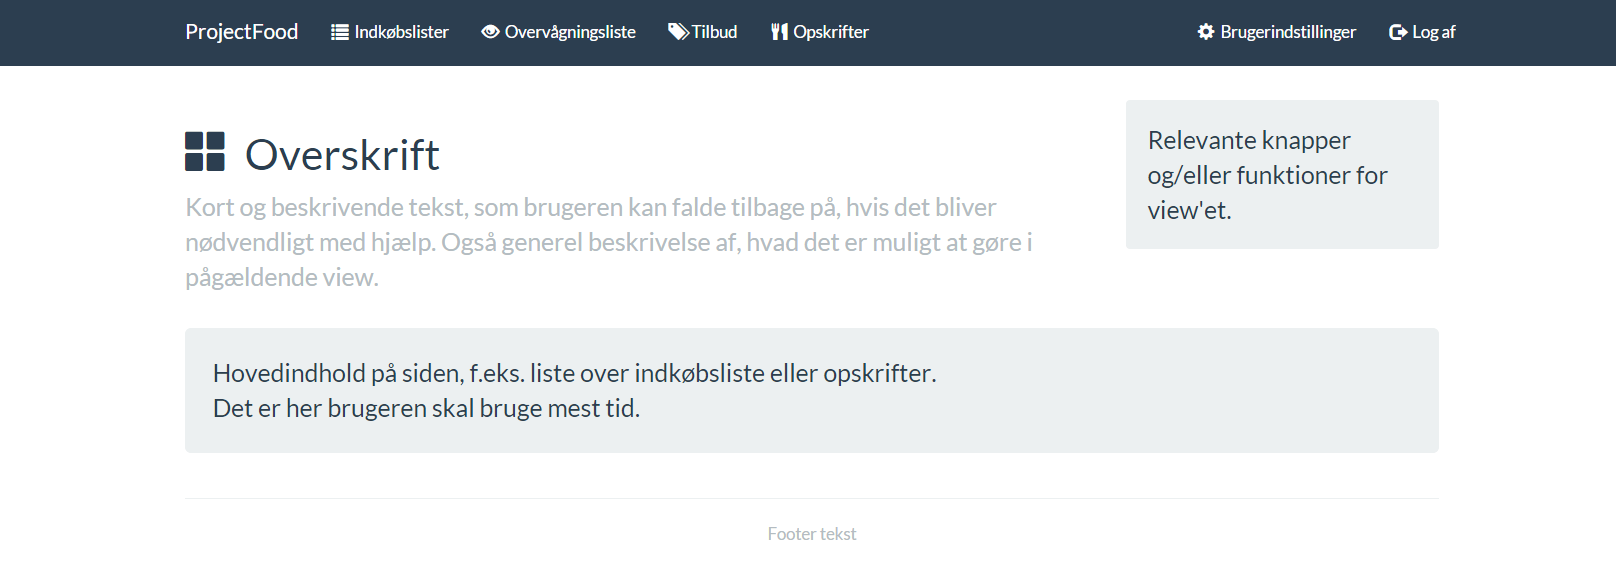
\includegraphics[trim=3.5cm 0cm 3cm 0cm, clip=true, width=1\textwidth]{images/Images/generelt_layout.png}
\caption{Design skabelon som beskriver den umiddelbare inddeling af views i systemet.}\label{ss:design_skabelon}
\end{figure}
Skabelonen er bygget op med tre hovedgrupper, foruden navigerings-baren og footeren. En gruppe til ikon(glyphicon), overskrift og forklarende hjælpetekst, en anden gruppe til knapper og relevante funktioner (det kunne f.eks. være en ``Opret indkøbsliste''-knap), og en tredje gruppe til selve hovedindholdet.
I HTML syntaks vil \myref{ss:design_skabelon}, se således ud:
\begin{lstlisting}[language=HTML, caption=HTML-kode med de tre hoved grupper, label=html:design_skabelon]
<div class="page-header nopadding-xs">
    <div class="container-fluid nopadding">
        <div class="col-md-9 col-xs-12 nopadding">
            <!--- Første gruppe --->
            <h1><span class="glyphicon glyphicon-th-large"></span>&nbsp;&nbsp;Overskrift</h1>
            <p class="hidden-xs lead text-muted nopadding">
                Kort og beskrivende tekst, som brugeren kan falde tilbage på, hvis det bliver nødvendligt med hjælp.
                Også generel beskrivelse af, hvad det er muligt at gøre i pågældende view.
            </p>
            <!--- Første gruppe slut --->
        </div>
        <div class="col-md-3 col-xs-12 nopadding">
            <!--- Anden gruppe --->            
            <div class="well lead">
                Relevante knapper og/eller funktioner for view'et.
            </div>
            <!--- Anden gruppe slut --->
        </div>
    </div>
</div>
<div class="container-fluid nopadding">
    <!--- Tredje gruppe --->
    <div class="well well-lg lead">
        Hovedindhold på siden, f.eks. liste over indkøbsliste eller opskrifter.<br />
        Det er her brugeren skal bruge mest tid.
    </div>
    <!--- Tredje gruppe slut --->
</div>
\end{lstlisting}

I HTML koden i \myref{html:design_skabelon} anvender Bootstrap klasser, resultatet kan ses \myref{ss:design_skabelon}. 
Gitter-systemet som Bootstrap stiller til rådighed bruges, for at få at opnå det ønsket layout og på samme tid tilpasses den mobil-platform.
Vi har udviklet vores egne CSS-klasser som f.eks. \texttt{nopadding}, for at kunne tilpasse layoutet yderligere. 
Med denne blanding af Bootstrap og vores eget CSS, kan vi tilpasse systemet præcis som vi vil. 
En af de andre funktioner, vi benytter fra Bootstrap, er \textit{glyphicons}, som øger hjemmesidens consistency og affordance.
Disse \textit{glyphicons} bruges bl.a. i overskrifter, og i navigerings-baren.

\textbf{Mobil tilpasning}\hfill\\
Det meste af vores tilpasning til mobil-platformen, klares af bootstaps responsive design, som er opnået ved at definere forskellige atributter for forskellige skærm størrelser.
Derudover benytter vi os af CSS-klasser, fra Bootstrap, som kan skjule og/eller vise ting ved netop forskellige skærm størrelser.
Vi vælger derved at begrænse systemets funktionalitet for brugeren, når de tilgår det via en mobil-platform. De funktioner, som vi skjuler for brugeren, er:

\begin{description}
\item[Oprettelse, redigering og kloning af opskrifter]\hfill\\
Grunden til, at vi har valgt at begrænse brugeren for denne funktionalitet på mobil-platformen, er at denne platform ikke er tænkt som et sted, hvor man skal foretage forholdvis kompliceret data oprettelse eller ændring.
Samtidigt fokuserer vi opskrifts komponenten omkring den relevate kontekst, når mobil-platforment benyttes, som er inspirationssøgning eller madlavning - i disse kontekster er det kun nødvendigt at kunne finde opskrifter og følge dem.
\item[Muligheden for at ændre kodeord]\hfill\\
Dette er ikke noget brugeren vil gøre ofte, og derfor har vi valgt, at ekskludere denne funktion fra mobil-platformen.
\end{description}

Når vi vælger at skjule funktionalitet for brugeren, er det udelukkende for at give brugeren en bedre oplevelse med brugen af hjemmesiden på mobil-platformen.
Vi påfører \textit{constraints} og på den måde, forhindres brugeren i, at tilgå steder der ikke egner sig til mobil-platformen.
Med fordel kunne man inkoorporere alle funktioner vha. \textit{overflow menuer} bl.a. kendt fra Google's tjenester, hvor tre prikker indikerer at yderligere funktionalitet er tilgængelig. \cite{actionbar}
På denne måde vil brugere, der udelukkende benytter sig at smartphones eller lign. også være i stand til at kunne udnytte alle hjemmesidens funktionaliteter.

\begin{wrapfigure}{o}{0.42\textwidth}
\vspace{-30pt}
\begin{center}
\textit{Desktop}
\frame{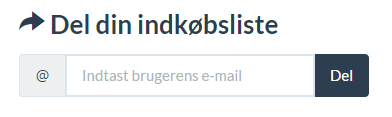
\includegraphics[width=0.4\textwidth]{images/Images/share_desktop.png}}\\
\vspace{10pt}
\textit{Mobil (efter tryk på knap)}
\frame{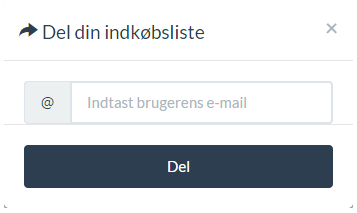
\includegraphics[width=0.4\textwidth]{images/Images/share_modal.png}}
\end{center}
\vspace{-10pt}
\caption{Her ses henholdsvis desktop- og mobil-udgaven af \textit{del-funktionen}}\label{ss:share_diffs}
\vspace{-30pt}
\end{wrapfigure}
Nogle steder har vi istedet for at gemme en funktionalitet væk, erstattet f.eks. en tekstboks med en knap, der så generere et vindue med de elementer der skal til for at udføre handlingen. 
Et eksempel på dette ses, når en bruger vil dele sin indkøbsliste med andre brugere.
På en computer vil man blive præsenteret for en tekstboks, med dertilhørende knap, mens mobil-udgaven viser brugeren en knap med titlen \textit{Del}, som generere et pop-up over selve siden, når de trykker på den (se \myref{ss:share_diffs} ).

\textbf{Respons til brugerinput}\hfill\\
For at brugeren oplever systemet som \textit{levende}, har vi implementeret forskellige former for respons og visuel feedback.
Dette gøres gennem jQuery og Bootstrap klasser.
Med Javascript og jQuery, kan man tilføje og fjerne klasser fra HTML tags, samt genere HTML kode uden at genindlæse siden - på den måde virker det for brugeren som om, at siden er \textit{levende}.
Vi har derudover valgt at benytte os af et javascript framework, kaldet \class{snackbar.js}, der tillader os, at præsentere brugeren for en snackbar.
En snackbar er, i dette tilfælde, en lille besked der popper op i nederste venstre hjørne af skærmen; snackbaren kan indeholde en hvilken som helst besked, og vi kan endvidere vise glyphicons deri.
Nogle eksempler på dette er:
\begin{description}
\item[Tilføje varer til indkøbsliste, fra tilbud side eller opskrift]\hfill\\
Ud for hvert tilbud, på tilbuds siden, og ingredienser på opskrifter, er det muligt for brugeren at trykke på en blå knap, der er præsenteret med et plus (\textbf{+}). 
Når varen bliver tilføjet, vil brugeren opleve, at knappen skifter farve til grøn, og plusset bliver til et flueben.
Derudover vil en snackbar komme til syne, med en besked om, at det er lykkedes at tilføje varen til den valgte indkøbsliste.
(Se \myref{code:user_feedback} funktion nr. 1)
\item[Ændre hvilke butikker man ønsker at se tilbud fra]\hfill\\
Under brugerindstillinger, er der ud for alle butikker vist en checkboks, som systemet har fundet tilbud fra.
Som udgangspunkt er alle butikker tilvalgt, hvilket er vist med et flueben i checkboksen.
Når brugeren så vælger at fjerne en butik, vil fluebenet forsvinde, og teksten bliver overstreget og faded ud.
Vi informerer også brugeren om, at indstillingen er gemt, med en snackbar.
(Variation af funktion nr. 1 på \myref{code:user_feedback})
\item[Dele indkøbsliste med andre brugere]\hfill\\
Hvis brugeren forsøger at dele sin indkøbsliste med en anden bruger, præsenterer vi resultatet af handlingen igennem en snackbar.
På denne måde kan brugeren se, om det er lykkedes eller om den indtastede email ikke findes.
(Udvidelse af funktion nr. 2 på \myref{code:user_feedback})
\end{description}

\begin{lstlisting}[language=JavaScript,caption={Javascript funktioner, der giver bruger feedback},label=code:user_feedback]
function ChangeToCheckRecipe(json) {
    var recipeButton = '#AddItem_' + json.itemID;
    $(recipeButton)
        .removeClass('btn-info')
        .addClass('btn-success')
        .blur();
    $(recipeButton + ' span')
        .removeClass('glyphicon-plus')
        .addClass('glyphicon-ok');
    MakeSnackbar("Vare tilføjet til " + json.shoppingListTitle, "glyphicon-ok", "toast", "1500");
};

//Generate snackbar and show on screen. text, glyphicon, style and timeout is optional.
function MakeSnackbar(text, glyphicon, style, timeout) {
    $('#snackbar-container').children().each(function () {
        $(this).snackbar('hide');
    });
    var options;
    if (isset(glyphicon)) {
        var glyphiconContainer = $('<div>');
        var span = $('<span>').addClass('glyphicon').addClass(glyphicon);
        glyphiconContainer.append(span);
        options = {
            content: glyphiconContainer.html() + "&nbsp;&nbsp;" + ((isset(text)) ? text : " "),
            style: (isset(style)) ? style : "snackbar",
            timeout: (isset(timeout)) ? timeout : 2500
        };
    } else {
        options = {
            content: (isset(text)) ? text : " ",
            style: (isset(style)) ? style : "snackbar",
            timeout: (isset(timeout)) ? timeout : 2500
        };
    }
    $.snackbar(options);
};
\end{lstlisting}

\subsection{Konklusion}
Med vores design skabelon og brugen af \textit{glyphicons}, forøger vi niveauet af \textbf{learnability} markant, og brugeren får i sidste ende lettere ved at bruge hjemmesiden.
For at opfylde kravet om \textbf{effectiveness}, benytter vi os af constraints, bl.a. begrænset funktionaliteterne i forskellige kontekster.
\textbf{Ease of use} opnås ved, at systemet giver brugeren feedback, når der foretages forskellige handlinger.
Her er muligheden for at lave \textit{snackbars} en essentiel del.
Brugen af vores design skabelon, samt navigerings-baren, hjælper også med til at overholde Getalts love om perception, i form af gruppering.
Guidelines omkring mobile-platforme, overholder vi bl.a. igennem overvejelser ift. konteksten i udviklingen af vores views.
Eftersom vi ikke har valgt at udvikle en dedikeret app, til smartphones, hjælper det også meget på brugeroplevelsen, at vi kan præsentere den mobile-udgave uden url-baren der normalt optræder i browseren.